\clearpage
\section{Discrete Variables Quantum Tx/Rx system - Physical Layer}

\begin{refsection}

\begin{tcolorbox}	
\begin{tabular}{p{2.75cm} p{0.2cm} p{10.5cm}} 	
\textbf{Student Name}  &:& Mariana Ramos\\
\textbf{Starting Date} &:& May 05, 2019\\
\textbf{Goal}          &:& Algorithm for polarization drift compensation with discrete variables.\\
\textbf{Directory}     &:& sdf/dv\_polarization\_encoding\_system.
\end{tabular}
\end{tcolorbox}



%%%%%%%%%%%%%%%%%%%%%%%%%%%%%%%%%%%%%%%%%%%%%%%%%%%%%%%%%%%%%%%%%%%%%%%%%%%%%%%%%%%%%%%%%%%%%%%%%%%%%%%%%%%%%%%
%%%%%%%%%%%%%%%%%%%%%%%%%Simulation Algorithm%%%%%%%%%%%%%%%%%%%%%%%%%%%%%%%%%%%%%%%%%%%%%%%%%%%%%%%%%%%%%%%%%%
%%%%%%%%%%%%%%%%%%%%%%%%%%%%%%%%%%%%%%%%%%%%%%%%%%%%%%%%%%%%%%%%%%%%%%%%%%%%%%%%%%%%%%%%%%%%%%%%%%%%%%%%%%%%%%%
\subsection{Simulation Analysis - Algorithm for polarization compensation}

\begin{figure}[h]
    \centering
        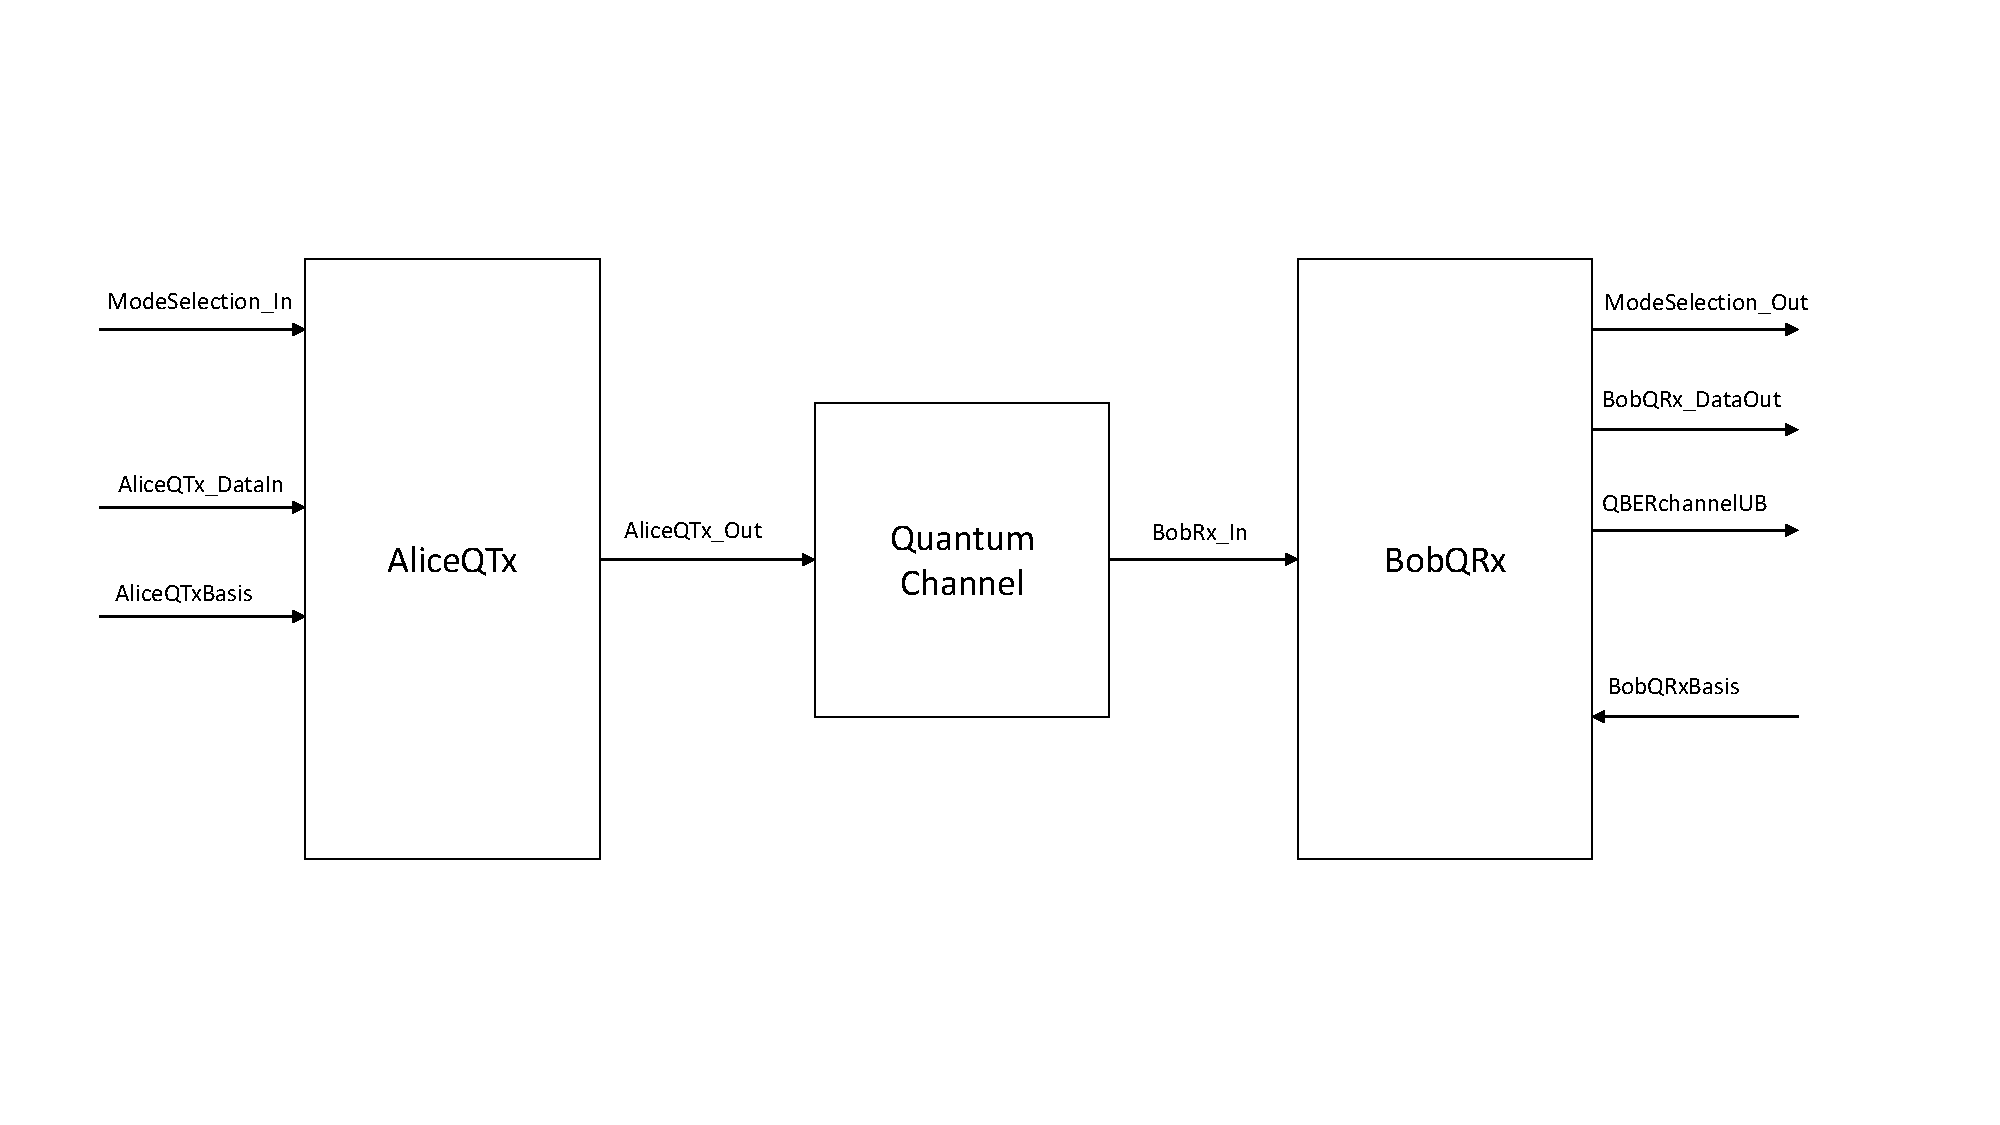
\includegraphics[clip, trim=1.6cm 3.0cm 3cm 2cm, width=0.80\textwidth]{./sdf/DvQuantumTxRx/figures/Diagram.pdf}
    \caption{Block diagram of a DV quantum Tx/Rx system to emulate the physical layer.}\label{dvquantumtxrx_diagram}
\end{figure}

This system emulates the physical layer of a quantum communication system. In this way, it comprises three super blocks. The first is the AliceQTx, which emulates the quantum transmitter of single-photons using polarization encoding. This block has three inputs: the ModeSelection, when it has value '0' selects the monitoring mode in which Alice transmits 1 control qubit in each \textbf{N} transmitted qubits. The remaining 99 qubits are data qubits which are encoded taking into account the other two inputs that are binary signals with basis, AliceQTxBasis, and other with the bit values, AliceQTxBits. Combining these two binary signals Alice is capable of encode 4 different states of polarization in two non-orthogonal basis in the photonStreamXY signal AliceQTxOut. When ModeSelection has the value '1' AliceQTx only transmits control qubits continuously according with a pre-defined sequence.
The super block quantum channel accepts and outputs a photonStreamXY signal, and intends to emulate the polarization random drift throughout the optical fiber and the attenuation induced by it. The super block BobQRx receives the photonStreamXY signal and will measure and decode the single photon. This block outputs a binary signal ModeSelection that later inputs Alice super block. It also outputs BobQRxDataOut, which is a signal with Bob's measurements. This is a real signal has five possible value: 5 if it is a control qubit, and the upper layer should simply discard it, 3 if no-click happened, 2 if both detectors clicked, 0 if bit zero was measured and 1 if bit one was measured. It also outputs a real signal with the quantum channel QBER, QBER\_Qchannel, and the ModeSelection. BobQRx accepts a binary signal, BobQRxBasis, which comprises the basis for data qubits measurements.

\subsection{Simulation Analysis - TestBench}

\begin{figure}[h]
    \centering
        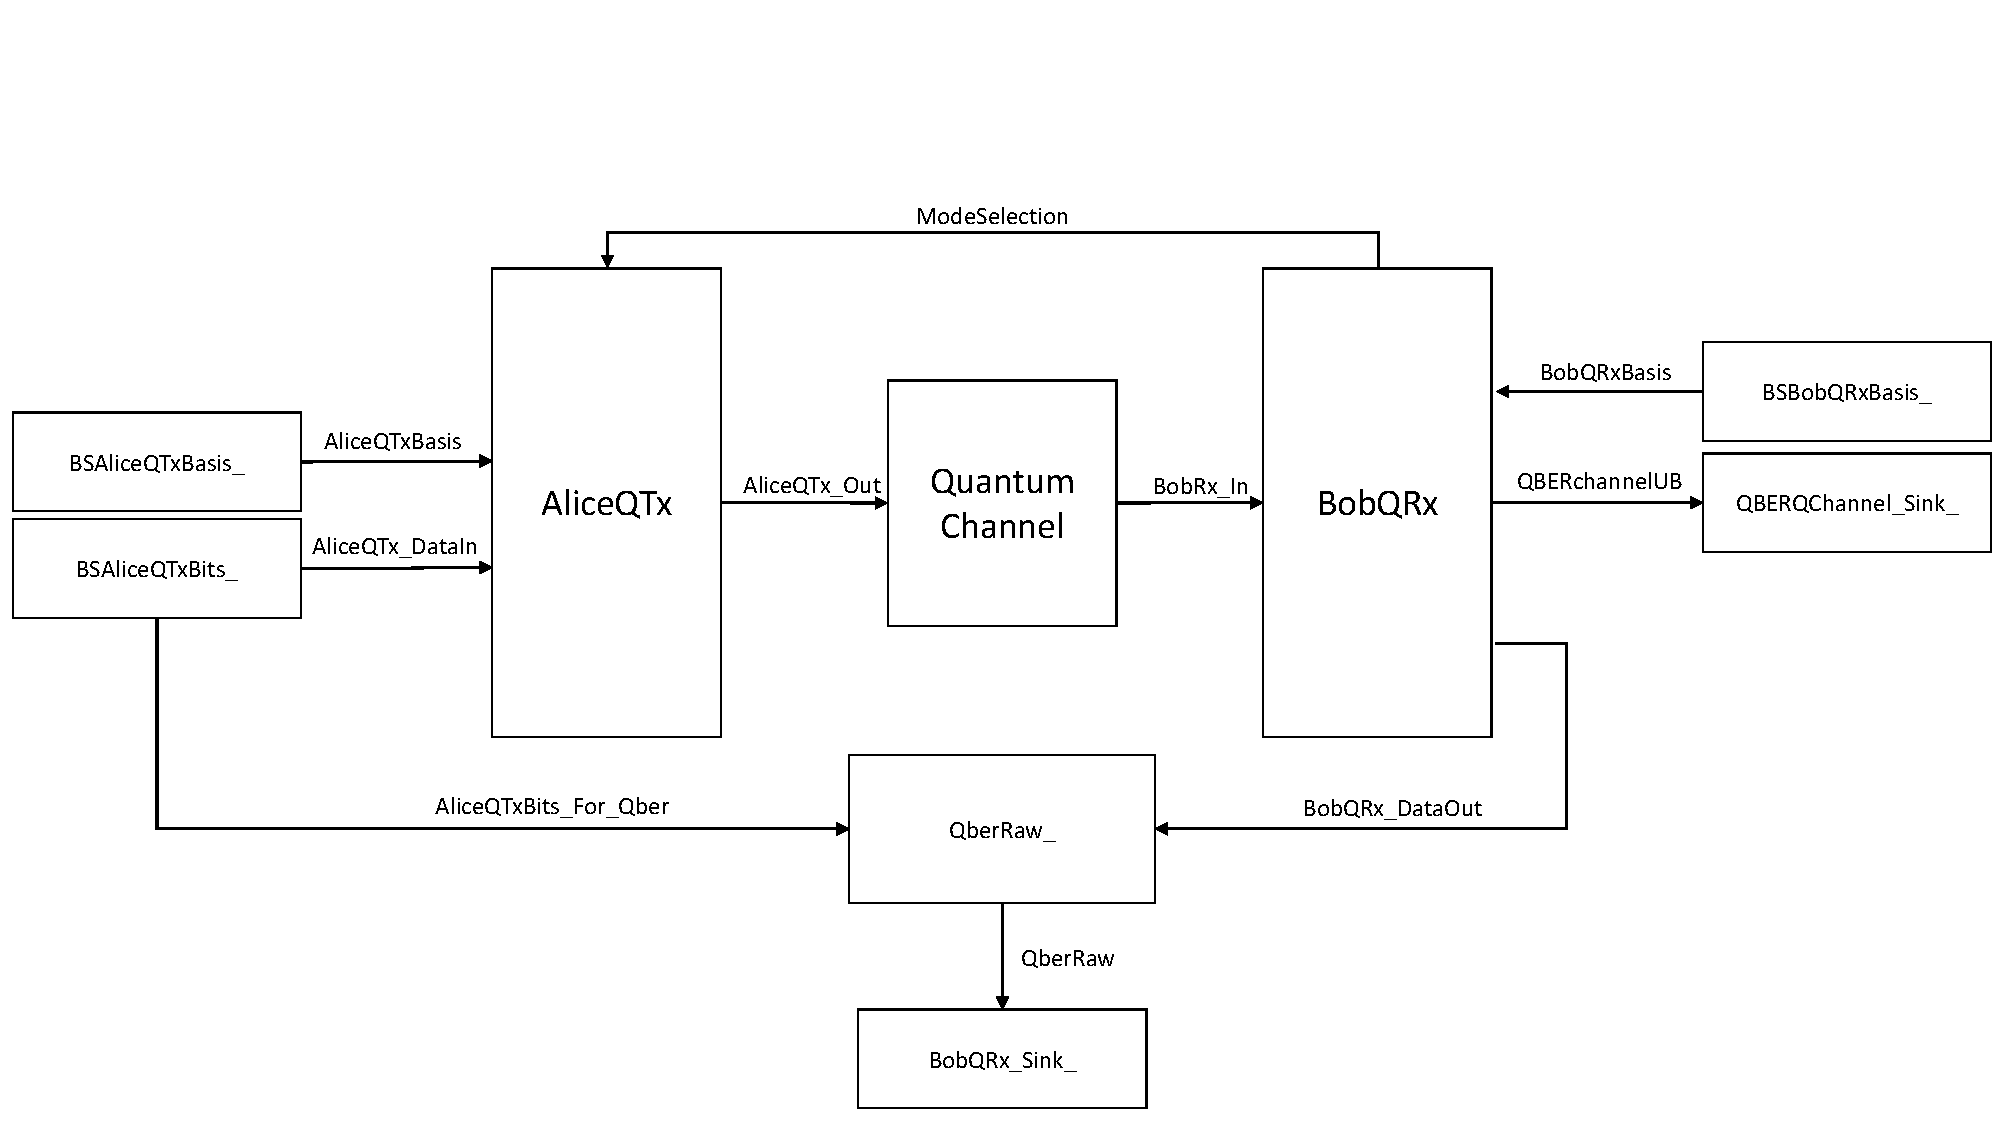
\includegraphics[clip, trim=0.1cm 0.1cm 0.1cm 2cm, width=0.80\textwidth]{./sdf/DvQuantumTxRx/figures/TesteBench.pdf}
    \caption{TestBench to test the DV quantum Tx/Rx system the physical layer emulator.}\label{testbench}
\end{figure}

This testbench was developed for testing the quantum physical layer presented in figure \ref{dvquantumtxrx_diagram}. In this way, the \textbf{modeSelection} signal was directly connected from \textbf{BobQRx} to \textbf{AliceQTx}. 

This system must be set with the following input parameters:

\begin{itemize}
  \item \textit{double} bitRate\{ 1e3 \},
  \item \textit{double} channelAttenuationDb\{ 0.2 \},
  \item \textit{sop\_rotation\_type} channelModel\{ sop\_rotation\_type::Stocastic \},
  \item \textit{double} PolarizationLinewidth\{ 900e-9 \},
  \item \textit{double} fiberLength\_km\{ 50 \},
  \item \textit{double} nPhotonsData\{ 1 \},
  \item \textit{double} nPhotonsControl\{ 80 \},
  \item \textit{int} nIncrementControl\{ 100 \}.
\end{itemize}

Furthermore, six more blocks were added with the following input parameters:

\begin{itemize}
  \item BSAliceQTxBasis\_:
    \begin{itemize}
      \item setMode(BinarySourceMode::DeterministicCyclic)
      \item setBitPeriod(1 / bitRate)
      \item setBitStream("1")
      \item setNumberOfBits(nBits);
    \end{itemize}

  \item BSAliceQTxBits\_:
    \begin{itemize}
      \item setMode(BinarySourceMode::DeterministicCyclic)
      \item setBitPeriod(1 / bitRate)
      \item setBitStream("0");
    \end{itemize}
    
  \item BSBobQRxBasis\_:
    \begin{itemize}
      \item setMode(BinarySourceMode::DeterministicCyclic)
      \item setBitStream("1")
      \item setBitPeriod(1 / bitRate);
    \end{itemize}
    
  \item QberRaw\_;
  
  \item BobQRx\_Sink\_;
  
  \item QBERQChannel\_Sink\_.
\end{itemize}

The three main blocks were defined with the following parameters:

\begin{itemize}
  \item AliceQTx\_:
    \begin{itemize}
      \item setControlBasisSequence("0")
      \item setControlBitsSequence("0")
      \item setNumberOfPhotonsData(nPhotonsData)
      \item setNumberOfPhotonsControl(nPhotonsControl)
      \item setIncrementControl(nIncrementControl);
    \end{itemize}
    
  \item QuantumChannel\_:
    \begin{itemize}
      \item setAtennuationDbmPerKm(channelAttenuationDb)
      \item setFiberLength(fiberLength\_km)
      \item setFiberModel(channelModel)
      \item setPolarizationLinewidth(PolarizationLinewidth);
    \end{itemize}
    
  \item BobQRx\_:
    \begin{itemize}
      \item setControlSequenceBits("0")
      \item setControlBasisMeasurement("0")
      \item setIncrementControl(nIncrementControl).
    \end{itemize}
\end{itemize}

\subsection{Open Issues}


% bibliographic references for the section ----------------------------
\clearpage
\printbibliography[heading=subbibliography]
\end{refsection}
\addcontentsline{toc}{subsection}{Bibliography}
\cleardoublepage
% ---------------------------------------------------------------------
